\section{Architecture}
Before diving into the code and its structure, let's take some time to understand how id's developers worked. Before \doom, all work was done on a PC. Code was written and compiled, and the resulting executable started on the same machine. With the introduction of \NeXT workstations into the mix, the process had to be different.\\
\par
A developer had two machines, a \NeXT workstation and a PC. All authoring work was done on the \NeXTns{}. Code was written with \cw{TextEdit.app}, compiled with \cw{gcc}, linked with \cw{ld}, and the executable ran on the NeXTstation. The biggest advantage of working on a Unix system was stability. Developers never lost their work due to IDE crashes\footnote{With Borland C++, crashes were a daily occurrence (source: correspondence with John Carmack).}.\\
\par
Once the developer was happy with the result, he switched to his second machine. In order to do so, he literally rolled his chair over to the PC where the \NeXT workstation's hard-drive was mounted over NFS. The PC compiled the same source code\footnote{With some platform specifics.} a second time with Watcom toolchain, \cw{WCC386.EXE} compiler and \cw{WLINK.EXE} linker, to generate \cw{DOOM.EXE}. \\
\par
 In this setup the PC was relegated to "only" running the game and assessing performance. The PC's hard-drive was actually used only to boot the machine and host the \cw{WATCOM} compiler. Everything else including the \cw{DOOM.EXE} executable was stored on the \NeXT SCSI HDD.\\
\par
There were significant obstacles to this methodology. First of all, DOS programs had direct access to the hardware whereas NeXT processes had to use "official" APIs. Second and perhaps most importantly, the two machines had different endianness. PCs ran on Intel CPUs which were little-endian whereas \NeXT machines used the big endian Motorola 68040 CPU.\\
\vspace{2mm}
\par
\begin{figure}[H]
\centering
\scaleddrawing{0.8}{dev_setup}{\protect\NeXT HDD user home folder is mounted on DOS machine as Z drive.}
\end{figure}
\par



\subsection{Solving Endianness}
Endianness was a term introduced by Danny Cohen in his essay "On holy wars and a plea for peace". His satire, based on Gulliver's Travels in which civil war erupts over whether the big end or the little end of a boiled egg is the proper end to crack open, made for an analogy between two schools of thought among CPU manufacturers. Some wanted bytes organized in memory from left to right, some wanted them right to left. Each side viewed their way as the best one.\\
\par
In a war where programmers paid the price, no side had any incentive toward peace.



The order of bits in a byte was in universal agreement, but the order of bytes in larger structure, such as shorts (16 bits) or ints (32 bits) was differently interpreted based on the vendor's internal architecture. The stream \cw{0x12}, \cw{0x34}, \cw{0x56}, \cw{0x78} can be interpreted in two ways. On an Intel little-endian machine, it will be become \cw{0x78563412}. On a Motorola big-endian machine, it will become \cw{0x12345678}.\\
\par
\drawing{endianness}{A tiny wiring difference results in a hard frontier between CPU words}
\par
At the game engine level, the problem was solved via a layer of indirection with a simple macro\footnote{As of 2018 it seems the holy war is finally over. The little-endian tribe of Intel, AMD, and ARM has won.}. When reading from disk, the engine always uses either the \cw{LONG} or \cw{SHORT} macro to interpret data.\\
\par
\ccode{big_little_endian.c}
\par
\ccode{LongSwap.c}
\par
Even though \doom{} was written first on a \NeXT, the platform intentionally placed itself at a disadvantage. Because players would use MS-DOS, data was stored in little-endian so \cw{LONG} and \cw{SHORT} macros translated to zero instructions on consumer Intel based hardware.


\subsection{Solving APIs}
Accommodating the need to run on different operating systems was more challenging. The solution was to have a common "core" that was platform agnostic. To perform I/O, the core would tap into sub-systems specific to the platform they targeted.\\
\par
\begin{figure}[H]
\centering
\includegraphics[width=.5\textwidth]{drawings/doom_arch.pdf}
\caption{\doom{}'s core and its I/O platform-dependent systems. Notice the similarities with the design of an operating system.}
\end{figure}
\par
In the case of the video system, it would be using the VGA hardware on MS-DOS but the \cw{NSWindow} API on \NeXT. A naive implementation would have required a function pointer acting as a layer of indirection to dispatch each I/O call. A better solution leveraged C's linking stage.\\
\par
 While building a C program, all compilation units (\cw{.c} files) are compiled independently. At the end of the compilation step, all \cw{.c} files have been transformed into object (\cw{.o}) files. Object files may reference each other but because they were created independently, they have "holes" called "unresolved symbols". To generate an executable, all objects are given to a linker which will recognize unresolved symbols from all objects and patch the holes.\\
 \par
 Taking the example of \cw{s\_sound.c} which is part of the core and looking at \cw{s\_sound.o}, we can see this translation unit uses functions such as \cw{I\_PlaySong} and \cw{I\_StartSound} which are defined in the platform-specific sound system.\pagebreak

Asking \cw{nm} for undefined symbols shows an object file's "holes".\\
 \par
\tcode{s_sound_linker.txt}
\par
After the linker is done, there are no more unresolved symbols. The final executable is ready to run.\\
\par
\drawing{linking}{Most of the \doom{} code is shared. Only a few files are platform specific.}




\pagebreak
\drawing{doom_code_arch}{\doom{} source code architecture}
\par
In white are the core components. In grey are the I/O systems which require platform-specific code. On DOS these are provided by six extra files: \cw{i\_main.c}, \cw{i\_ibm.c}, \cw{planar.asm}, \cw{i\_ibm\_a.asm}, \cw{i\_sound.c}, and \cw{i\_cyber.c}.\\







\fullimage{Doom_build_NeXTStep.png}
\smallfakedosoutput{dos_compilation2.txt}


\vspace{-4mm}
\trivia{A full DOS build took an average of 3m19s. Linking alone took 19 seconds. Even incremental builds were time-consuming (e.g: change \cw{r\_sky.c} = 27s).}\\
\par
Notice the prefixed file name in figure \ref{doom_code_arch}. Since C has no namespaces, these prefixes are also applied to function names. \cw{I\_} stands for "implementation-specific", \cw{P\_} gameplay, \cw{R\_} is for renderer and so on.\\

The beauty of this architecture is that once the platform-specific systems are written, there is zero overhead to writing code that runs on multiple platforms. Most of the code goes into the core and the platform-specific code needs not be touched any more.\\
\par
Because portability was not an afterthought but an integral part of the development process, \doom{}'s code layering is never violated. This rigorous design partly explains why \doom{} has been ported to so many systems: there is very little code to write\footnote{"I ported DOOM to the Nintendo Switch in 45 minutes" by Modern Vintage Gamer on \cw{youtube.com}.}.\\
\par 
Additionally, working with multiple compilers such as gcc and Watcom not only surfaced many bugs, it also ensured the code would be ANSI standard compliant.\\
\vspace{-15pt}
\section{Diving In!}
Just before finally jumping in, here are a few stats gathered with the \cw{cloc} tool, just to know what volume of code to expect. There is roughly 40\% more code than in Wolfenstein 3D.\\
\par
\tcode{cloc.txt}
\par

\par
\begin{figure}[H]
\centering
  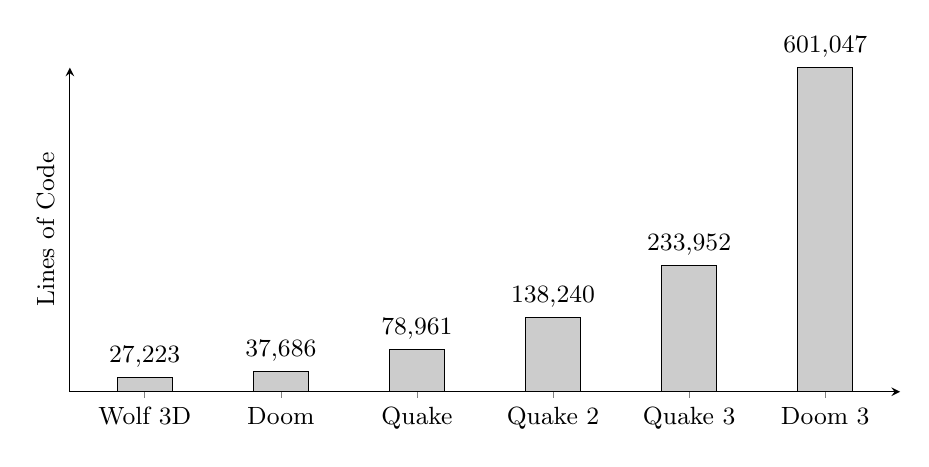
\begin{tikzpicture}[font=\small]
    \begin{axis}[
      width=\textwidth,
      height=0.47\textwidth,
      ybar=0.6\textwidth,
      bar width=20pt,
      ylabel={Lines of Code},
      ymin=0,
      ytick=\empty,
      xtick=data,
      axis x line=bottom,
      axis y line=left,
      enlarge x limits=0.11,
      symbolic x coords={Wolf 3D,Doom,Quake,Quake 2,Quake 3, Doom 3},
      xticklabel style={},
      yticklabel style={},
      nodes near coords={\pgfmathprintnumber[fixed,precision=0]\pgfplotspointmeta}
    ]
      \addplot[fill=black!20,draw=black] coordinates {
        (Wolf 3D,27223)
        (Doom,37686)
        (Quake,78961)
        (Quake 2, 138240)
        (Quake 3, 233952)
        (Doom 3, 601047)
      };
    \end{axis}
   \end{tikzpicture} 
   \caption{Lines of code from id Software game engines.}
 \end{figure}
\par

\subsection{Where Is My Main?}
Exploring a source code repository always starts with finding out what the OS will select as the entry point. 99\% of the time it means finding the \cw{int main(int,char**)} function\footnote{Of course, it is different on Microsoft Windows and you have to search for \cw{WinMain().}}. In the case of \doom{} there is one entry point per OS and they are all in implementation-specific (\cw{I\_*}) files. For DOS it is in \cw{i\_main.c}\footnote{On \NeXT the \cw{main} function is located in \cw{Doom\_main.m} and all it does is load "DoomRef.nib" into the window system.}.\\
\par
Regardless of the platform, all entry points converge on the core main function named \cw{D\_DoomMain} located in \cw{d\_main.c}.\\ 
\par

 \begin{figure}[H]
\centering  
\begin{tabularx}{\textwidth}{ L{0.22} C{0.39} C{0.39} }
  \toprule
  \textbf{System} & \textbf{DOS Implementation} & \textbf{NeXT Implementation}\\
  \toprule 
    Video System & VGA & NSWindow/libinterceptor\\
    Audio System & DMX & Not Implemented\\
    Control System & DPMI Interrupts & NSWindow/NXEvent \\
    File System & WAD/ endian macros & WAD/ endian macros\\
    Network System & Direct interrupts & BSD socket \\
    RAM System & greedy malloc & tight 4 MiB malloc\\
   \toprule
\end{tabularx}
\caption{Platform code specific.}
\end{figure}

\par

\trivia{\NeXT platform-specific code was written in Objective-C. All code was in five files named \cw{DRCoord.m}, \cw{VGAView.m}, \cw{Doom\_main.m}, \cw{i\_next.m}, and \cw{r\_debug.m}.}\\
\ccode{main.c}
\par
\ccode{main_loop.c}
\par
No surprises in \cw{D\_DoomMain}, the engine begins by initializing all its sub-systems before jumping to a loop which will never return (\cw{D\_DoomLoop}).\\
\par
Prefixes on translation units (and function names inside them) help to build a mental map of the various sub-systems. \cw{V\_} is for Video, \cw{M\_} is for Menu, \cw{Z\_} is for Zone Memory Allocator, \cw{R\_} is for Renderer, \cw{P\_} is for gamePlay, \cw{I\_} is for Implementation dependent, \cw{D\_} is for main Doom, \cw{S\_} is for Sound, \cw{HU\_} is for HUD, and \cw{ST\_} is for STatus bar.\\
\par
The developers did not try to hide what was going on during startup. \doom's openness needed no splash screen. The text mode messages show the player what is going on behind the scenes (figure \ref{dosloading}). For each initializer a line is output to the extent that the DOS screen on the right closely mirrors the source code in \cw{D\_DoomMain}.\\
\par
The startup step was fairly fast except for the excruciating renderer initialization in \cw{R\_Init} which took forever to complete. It featured not only a line but also a progress bar made up of dots which often required up to a minute to complete on the full version depending on the machine's hard drive access time. The details and meaning behind each dot are explained in the appendix on page \pageref{dots_explained}.\\
\par
\trivia{The \cw{-devparm} command line parameter shows more text output. One of these is "\cw{I\_StartupSound: Hope you hear a pop}"~which refers to the sound old speakers emitted when they were turned on. In an era before Plug\&Play and the Internet, it was an achievement itself to configure the sound card's mysterious IRQ and DMA parameters.}\\
% \par
\begin{figure}[H]
\fakedosoutput{doom_dos_start.txt}
\caption{DOS output upon starting \cw{DOOM.EXE}}
\label{dosloading}
\end{figure}

\par
\vspace{-10pt}
The game engine executable which shipped with the registered version of the game was the same that shipped with the shareware version. Two functions, \texttt{\justify FindResponseFile} and \cw{IdentifyVersion}, simply looked for the asset file and switched a flag depending on what WAD had been found (\cw{DOOM1.WAD} or \cw{DOOM.WAD}).
% \trivia{\doomii{} was officialy translated to another languge! A hard-coded \cw{doom2f.wad} is listed in the code which mean there a French version released at some point. Given the small market, it is surprising id went to the effort of translating the game.}




\section{Fixed Time Steps}
Peeking inside \cw{D\_DoomLoop} reveals a standard loop where the machine runs as fast as possible to update the game simulation according to user input and A.I., and then generate visual and audio output.\\
\par
\ccode{doomloop.c}
The game simulation happens in \cw{TryRunTics} and uses fixed time steps. The body of the function is summarized as follow:\\
\par
\ccode{TryRunTics.c}\label{TryRunTics.c}\\
\par
\doom's unit of time is the \cw{tic}. There are 35 tics in a second (which means a tic is 28ms) and 
\cw{I\_GetTime}'s clock unit is also the tic. On each iteration of \cw{D\_DoomLoop} the engine calculates how many tics have elapsed and advances the simulation by that amount. Only fully-elapsed tics are simulated. The value of 35 was not random; it is half the frequency of the VGA mode-Y. Once the game state has been updated, video and audio are generated.\\
\par
\drawing{fixed}{}
\par
This design choice would end up being controversial. On the one hand it solved the issue of recording a game session and being able to play back on any machine without desync. It also enabled network play and multiscreen play. On the other hand, it meant that no matter how fast the renderer could run, the game would only update at 35Hz which capped the visible framerate on the next generation of PCs based on Pentium CPUs.\\
\par



\section{Game Thread/Sound Thread}
MS-DOS did not support processes or threads, yet video and audio had to happen in parallel. To make this happen, the audio system is based on interrupts generated at a regular interval. This is explained in detail in the audio section on page \pageref{dmx_section}.\\
\scaleddrawing{0.9}{three_systems}{}
To disable register caching (resulting in infinite loops), the variable written by the sound engine and read by the \doom{} engine is declared \cw{volatile int ticcount}.







\section{Fixed-point arithmetic}
Since the Intel 486 CPU was unable to execute floating-point instructions fast enough, the programmers had to find a way to manipulate and store fractional values during calculations. The answer to this problem was to use fixed-point arithmetic.\\
\par
Designers at Intel had designed their CPUs to manipulate two types of 32-bit integers. In unsigned integers each bit represents a value from $0$ to $2^{32}-1$ for a decimal range of [0 to 4,294,967,295].\\
\par
\begin{figure}[H]
 \centering
  \input{drawings/uint.tex}
 \caption{32-bit unsigned integer bit values} 
\end{figure}
\par
Signed integers use two's complement where all bits represent a positive value except for the last one which is a negative value. Signed integers are able to represent values from $-2^{31}$ to $2^{31}-1$ yielding a decimal range of [-2,147,483,648 to 2,147,483,647].\\
\par
\begin{figure}[H]
 \centering
  \input{drawings/int.tex}
 \caption{32-bit signed two's complement bit values} 
\end{figure}
\par


For certain types of calculations, \doom{} resorts to using a different layout. The signed fixed-point format used is \cw{16:16} where bit 31 encodes a negative integer ($-2^{15}$), bits [30-16] store a positive integer, and bits [15-0] are used to store the fractional part. The decimal range is [-32768.0 to 32767.9999847]\footnote{All 32 bits set to 1 is the maximum value where the negative bit ($-2^{15}$) = -32768 is added to the positive values:  
 ($2^{14} + 2^{13} + 2^{12} + 2^{11} + 2^{10} + 2^9 + 2^8 + 2^7 + 2^6 + 2^5 + 2^4 + 2^3 + 2^2 + 2^1 + 2^0 + 2^{-1} + 2^{-2}+ 2^{-3}+ 2^{-4}+ 2^{-5}+ 2^{-6}+ 2^{-7}+ 2^{-8}+ 2^{-9}+ 2^{-10}+ 2^{-11}+ 2^{-12}+ 2^{-13}+ 2^{-14}+ 2^{-15}+ 2^{-16}$) = 32767.9999847.}.\\
\par
\begin{figure}[H]
 \centering
  \input{drawings/fp.tex}
  \caption{32-bit \doom{} fixed-point bit values}
\end{figure}
\par 
To help differentiate "regular" variables from "fixed-point" variables, a simple typedef \cw{fixed\_t} is used.\\
\par
\ccode{fixed_t.c}{}\\
\par
The beauty of the fixed-point system is that it "just works" at the ALU level -- the CPU executes instructions the same way. To convert from one type to another is very simple. From integer to fixed point is a cheap "\verb!<< 16!" bitwise left shift. From fixed point to integer is the reverse operation, a "\verb|>> 16|" bitwise right shift.\\
\par


As an example, $0.5 + 3.75 = 4.25$ yields the correct result bitwise.\\
\par
\begin{figure}[H]
  \centering
  \input{drawings/fp05.tex}
  \caption{Fixed-point representation of \cw{0.5}}
\end{figure}
\begin{figure}[H]
  \centering
  \input{drawings/fp375.tex}
  \caption{Fixed-point representation of \cw{3.75}}
\end{figure}
\begin{figure}[H]
  \centering
  \input{drawings/fp425.tex}
  \caption{Fixed Point representation of \cw{4.25}}
\end{figure}
\par
Even bitwise operations work such as fast divide/multiply with left shift ("\verb!<<!") and right shift ("\verb|>>|").\\
\par
\begin{figure}[H]
  \centering
  \input{drawings/fp85.tex}
  \caption{Fixed Point representation of \cw{4.25 << 1} = 8.5}
\end{figure}
\par

There are only two limitations to this system:
\begin{itemize}
  \item Contrary to floating point, there is no sliding window compensation to avoid overflow and adjust precision. Overflows have to be avoided otherwise information is lost (there are display bugs with extremely large maps caused by this specific problem). 
  \item Integers and fixed-point variables cannot be mixed during operations. The programmer has to manually convert from one to the other since the C language will not "promote" types automatically.
\end{itemize}
 

% Additions and Substractions work as usual but multiplication is a special case. Multiply two 32-bit value result in a 64-bit value which is shifted right 16-bit and clipped to 32-bit. This can result in an annoying lose of precision if data was in bits [16-0]and a potentially catastrophic lose of information if data was in bits [63-48]. Again, floating point unit operating at 80-bit precision avoid this but there is no such thing in fixed point.

\pagebreak

